\begin{figure*}[!tb]
\centering
\begin{subfigure}[t]{0.48\textwidth}
    \centering
    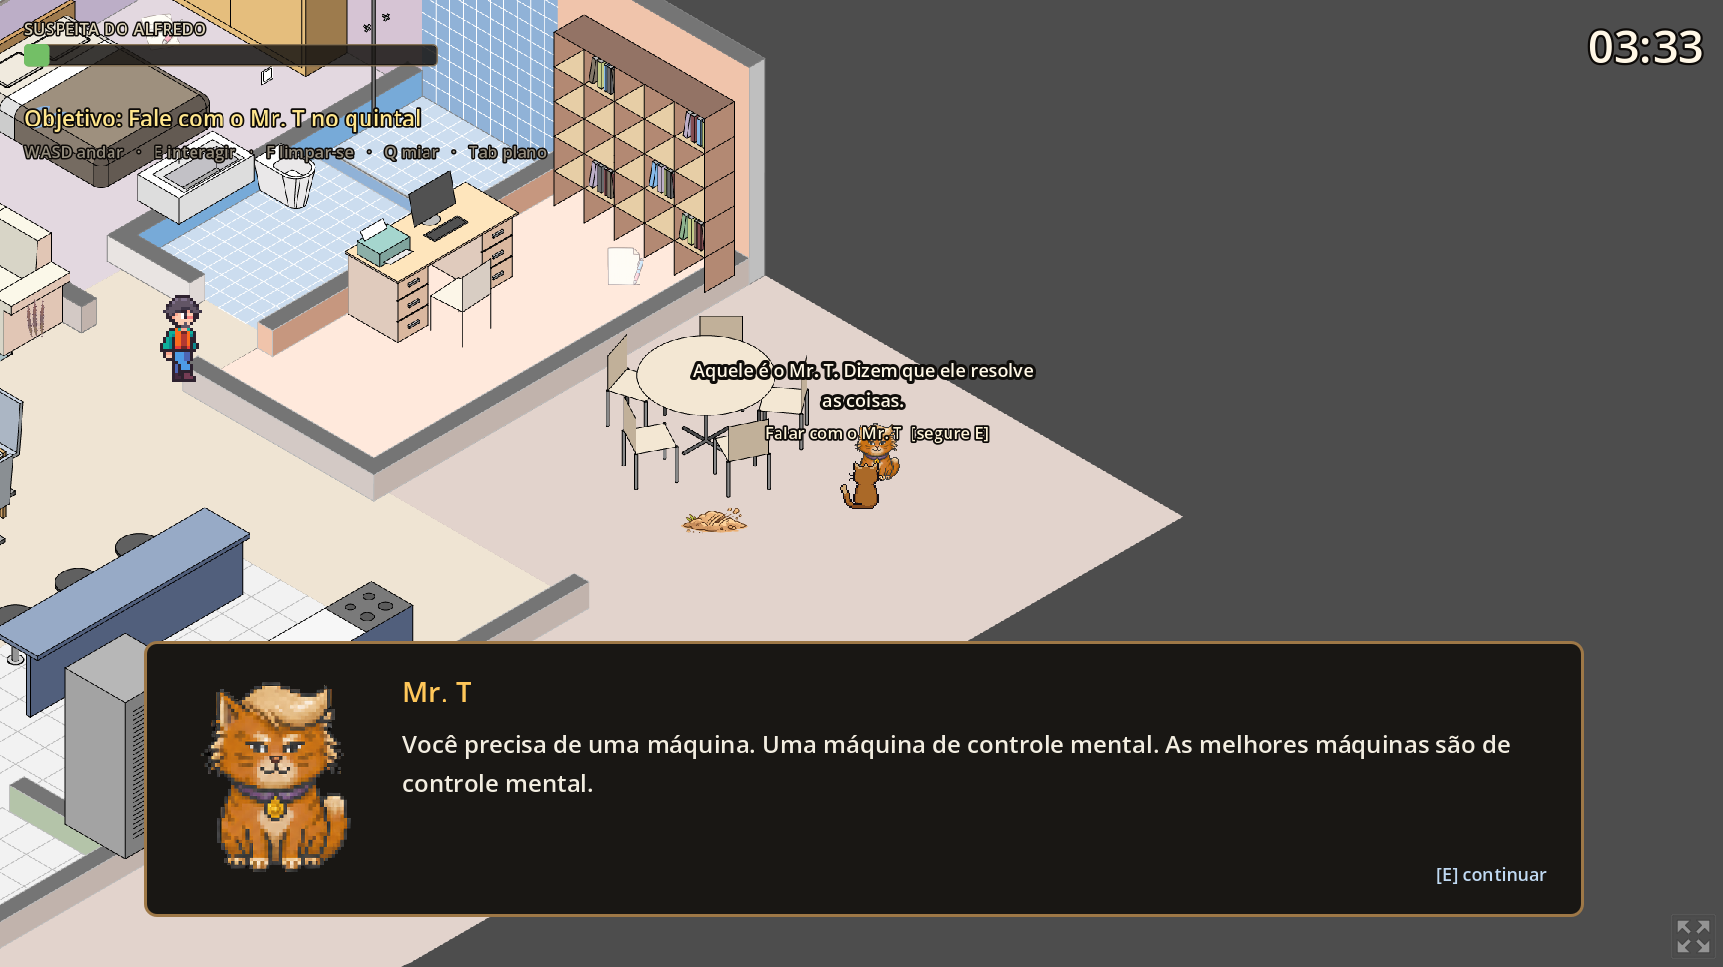
\includegraphics[width=\linewidth]{figures/mr_t.png}
    \caption{Interação inicial com Mr. T.}
    \label{fig:mr_t}
\end{subfigure}
\hfill
\begin{subfigure}[t]{0.48\textwidth}
    \centering
    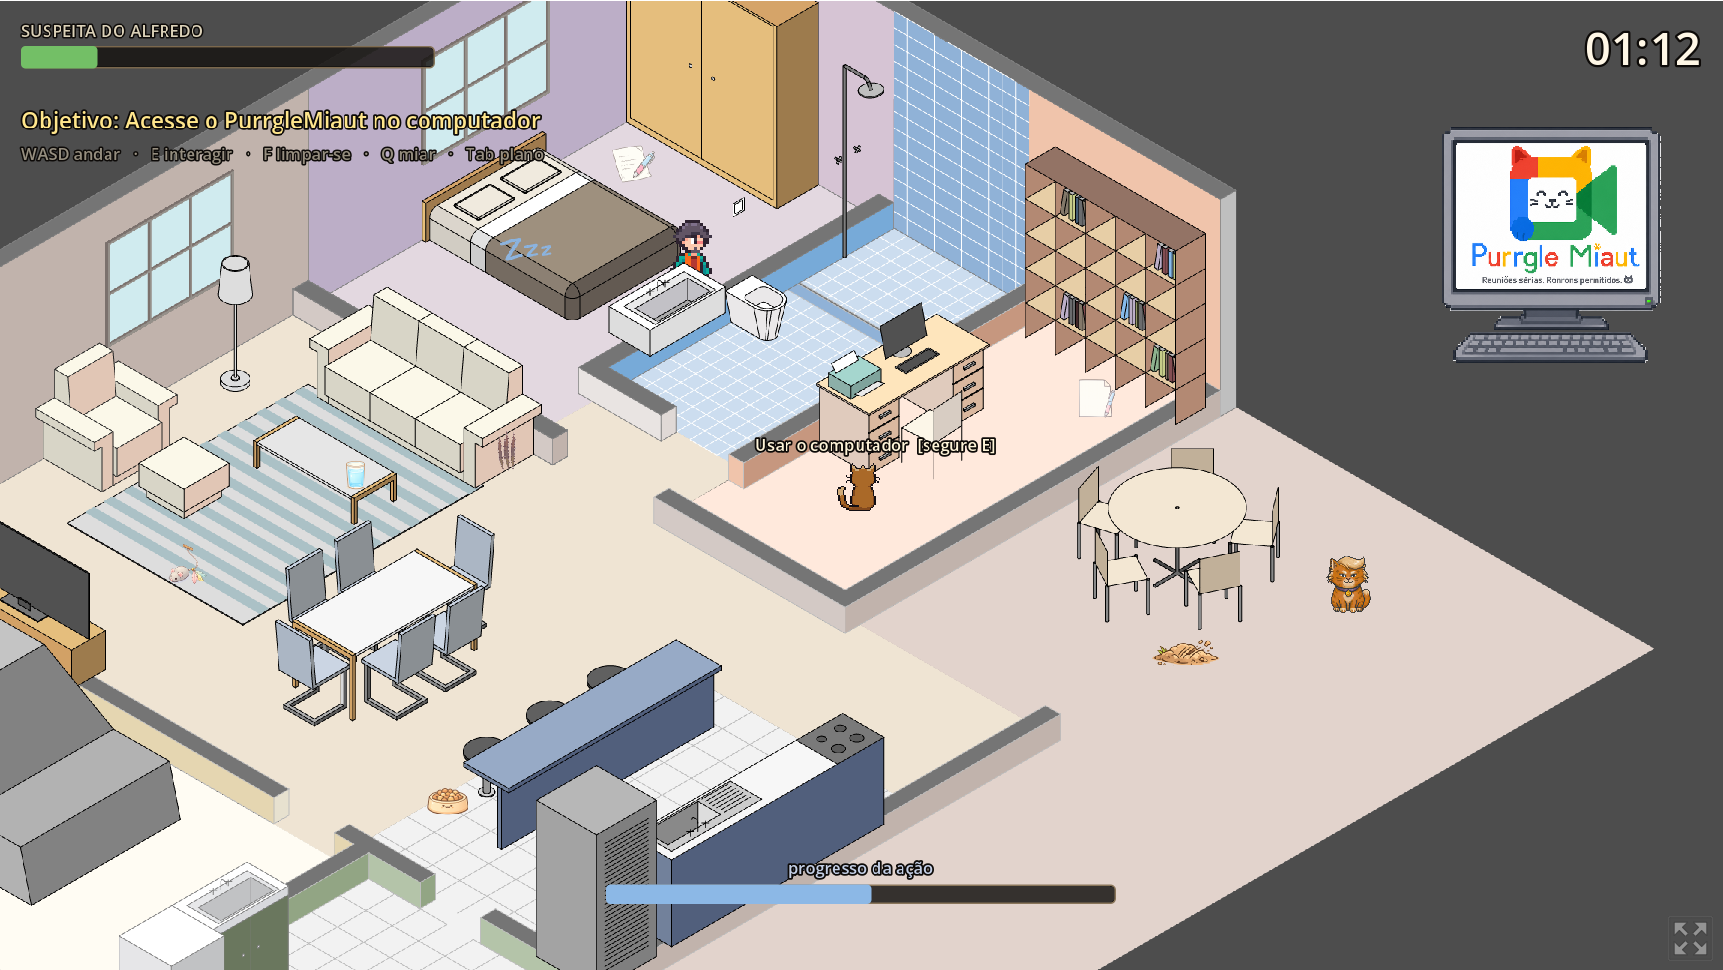
\includegraphics[width=\linewidth]{figures/purrgle_miaut.png}
    \caption{Busca de informações no Purrgle Miaut.}
    \label{fig:purrgle_miaut}
\end{subfigure}

\vspace{\baselineskip}

\begin{subfigure}[t]{0.48\textwidth}
    \centering
    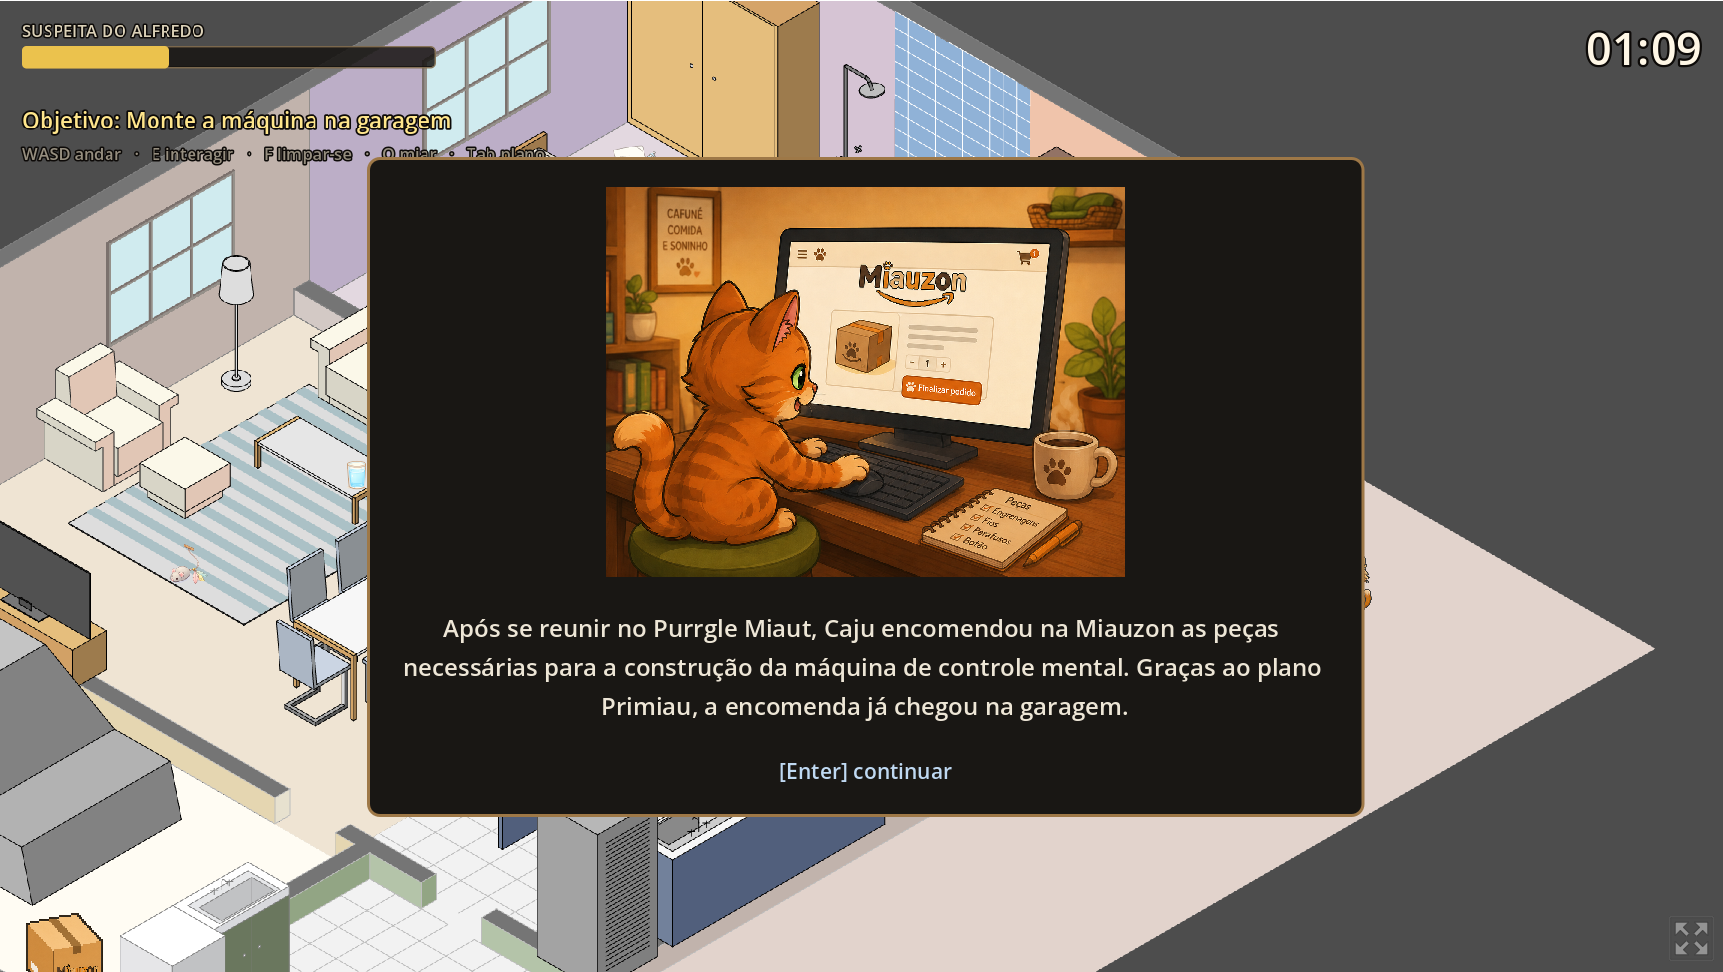
\includegraphics[width=\linewidth]{figures/miauzon.png}
    \caption{Conclusão da tarefa no Purrgle Miaut.}
    \label{fig:miauzon}
\end{subfigure}
\caption{Exemplos da progressão por tarefas ao longo da partida.}
\label{fig:tarefas}
\end{figure*}
